\documentclass[tikz,border=8pt]{standalone}
\usetikzlibrary{calc}
\begin{document}
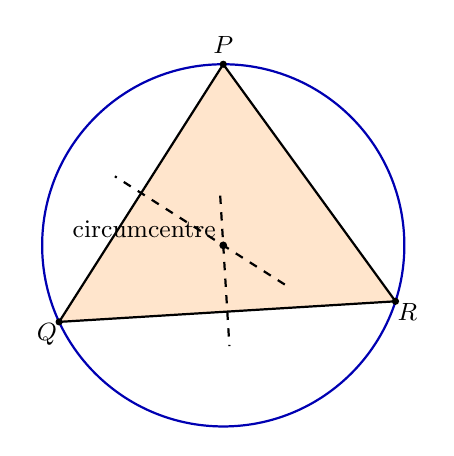
\begin{tikzpicture}[line width=0.8pt, font=\small]
  \coordinate (Ce) at (0,0);
  \coordinate (P) at (90:2.3);
  \coordinate (Q) at (205:2.3);
  \coordinate (R) at (342:2.3);
  \draw[blue!70!black] (Ce) circle (2.3);
  \fill[orange!20] (P) -- (Q) -- (R) -- cycle;
  \draw (P) -- (Q) -- (R) -- cycle;
  \coordinate (M1) at ($(P)!0.5!(Q)$);
  \coordinate (M2) at ($(Q)!0.5!(R)$);
  \draw[dashed] ($(M1)!1.75!(Ce)$) -- ($(Ce)!1.32!(M1)$);
  \draw[dashed] ($(M2)!1.75!(Ce)$) -- ($(Ce)!1.52!(M2)$);
  \fill (Ce) circle (1.4pt) node[above left=-1pt] {circumcentre};
  \fill (P) circle (1.3pt) node[above] {$P$};
  \fill (Q) circle (1.3pt) node[below left=-3pt] {$Q$};
  \fill (R) circle (1.3pt) node[below right=-3pt] {$R$};
\end{tikzpicture}
\end{document}
